\subsection{Parallel computing experiments}

Because one of the most crucial points of SMODERP2D computations is
the speed, an experimental branch allowing (both CPU and GPU-based)
parallelised computations has been developed.

The main step was to rewrite all loop-based computations into
matrix-based mathematical operations. To keep matrices as so-called
tensors and to perform all the operations, an open source Python
%% TODO: Ondra
library TensorFlow developed by Google Brain Team was used \cite{xxx}.
Even though TensorFlow is most widely used for machine learning and
its performance on basic mathematical operations is not always better
than the one of NumPy, it had been preferred for its easy switch
between CPU and GPU-based core (it depends only on the version of
TensorFlow the user has installed, no needs for changes in code) and
therefore support also for users without an access to machines with
GPU. Another advantage of TensorFlow is its usage of so-called
graphs. A graph is a representation of all operations in
dataflow/workflow and its individual operations are automatically sent
to multiple cores in a CPU or multiple threads in a GPU. These nodes
are run independently in parallel.

To support further development of TensorFlow and exploit its bleeding
edge functionalities, TensorFlow 2.0, which is published currently
just as an alpha version, was used in the SMODERP2D experimental
branch. Because TensorFlow 2.0 is still not suitable with all the
Python acrobatic tricks, NumPy was used for matrix operations in
places where TensorFlow could not (on places where loops were still
needed; looping through a NumPy array is incomparably faster than
through a Tensor).

This experimental SMODERP2D branch is still under development;
however, the alpha-version is ready to be used. Table \ref{tab:GPU_results}
presents the results of different tests made on this version.

\begin{table}[h]
  \centering
  \caption{Results of parallelization tests}
  \makegapedcells
  \begin{tabular}{|l|p{2.2cm}|c|c|}\hline
    RAM & Processing unit & Data 62 KB & Data 197 MB\\
     & & [s] & [s]\\\hline
    \multirow{2}{*}{15 GB} & GPU1 & 4.0 & 7 560\\
    & CPU1 & 0.2 & 12 809\\\hline
    \multirow{2}{*}{251 GB} & GPU2 & 2.5 & 8 631\\
    & CPU2 & 0.2 & 10 637\\\hline
  \end{tabular}
  \label{tab:GPU_results}
  \caption{Used processing units}
  \begin{tabular}{|l|p{1.9cm}|c|c|}\hline
    ID & Model & Clock speed & Memory\\\hline
    GPU1 & GeForce GTX 1060 3GB & 33 MHz & 3 016 MiB \\\hline
    GPU2 & 4x GeForce GTX 1080 Ti & 33 MHz & 11 178 MiB \\\hline
    CPU1 & AMD Ryzen 7 1700 Eight Core Processor & 1 373 MHz & 512 KB \\\hline
    CPU2 & Intel Xeon CPU E5-2630 v4 @ 2.20 GHz & 2 423 MHz & 25 600 KB \\\hline
  \end{tabular}
\end{table}

\subsubsection{Further ideas for a basins-based parallel computing}
Besides the GPU-based parallelization (with TensorFlow \cite{xxx} or
NVIDIA Cuda technology~\cite{Kalyanapu2011,Le2015}) the
CPU-parallelization may also bring a good improvement in the computation
time reduction. The computation domain is separated into sub-domains
based on certain algorithm were each sub-domains is loaded to single
CPU core. The domain may be separated into sub-domain with equal area
based on a defined grid. It is beneficial to incorporate also
hydrological behavior in the parallelization
strategy. In~\cite{Vivoni2011} the basins was separated in sub-basins
based on stream network. The sub-basins communicated with so called
ghost cell with each other where the water flowed between
sub-basins. The strategy aimed to generate as less ghost cells as
possible.

The parallelization strategy outlined in the manuscript is based on
the hydrological reality and it is depicted in a simplified setup in
the Figure~\ref{fig:cpu-parallel}. The strategy main goal is to reduce
the communication CPU-cores during the computation as much as
possible. The whole basin is divided into several sub-basins based on
the digital elevation model. Outlet of each sub-basin is depicted with
red dots in the Figure~\ref{fig:cpu-parallel}. After the sub-basins
are defined an order in which to be computed is defined as
follows. Sub-basins which are hydrologically the farthest from the
basin outlet and therefore have no inflow flow upslope catchments are
calculated at first. Those sub-basins have the rainfall recorded in
hyetograph as the only input. In the simplified setup shown in the
Figure~\ref{fig:cpu-parallel}, the sub-basins 1, 2, 3, and 6 are
calculated at first in parallel. The calculated hydrographs of the
sub-basins 1, 2, 3, and 4 are stored in the memory. Sub-basins which
has an inflow from sub-basins 1, 2, 3, and 6 are calculated next. It
this case it is only the sub-basin 4. In this case the water input in
the calculation are, besides the hyetograph, also hydrographs of
sub-basins 1 and 3 which flow in the basin 4. This the same manned are
calculated sub-basins towards in the outlet. (to be finished).

(add about possible advantages and disadvantages)

\begin{figure}[ht!]
  \begin{center}
    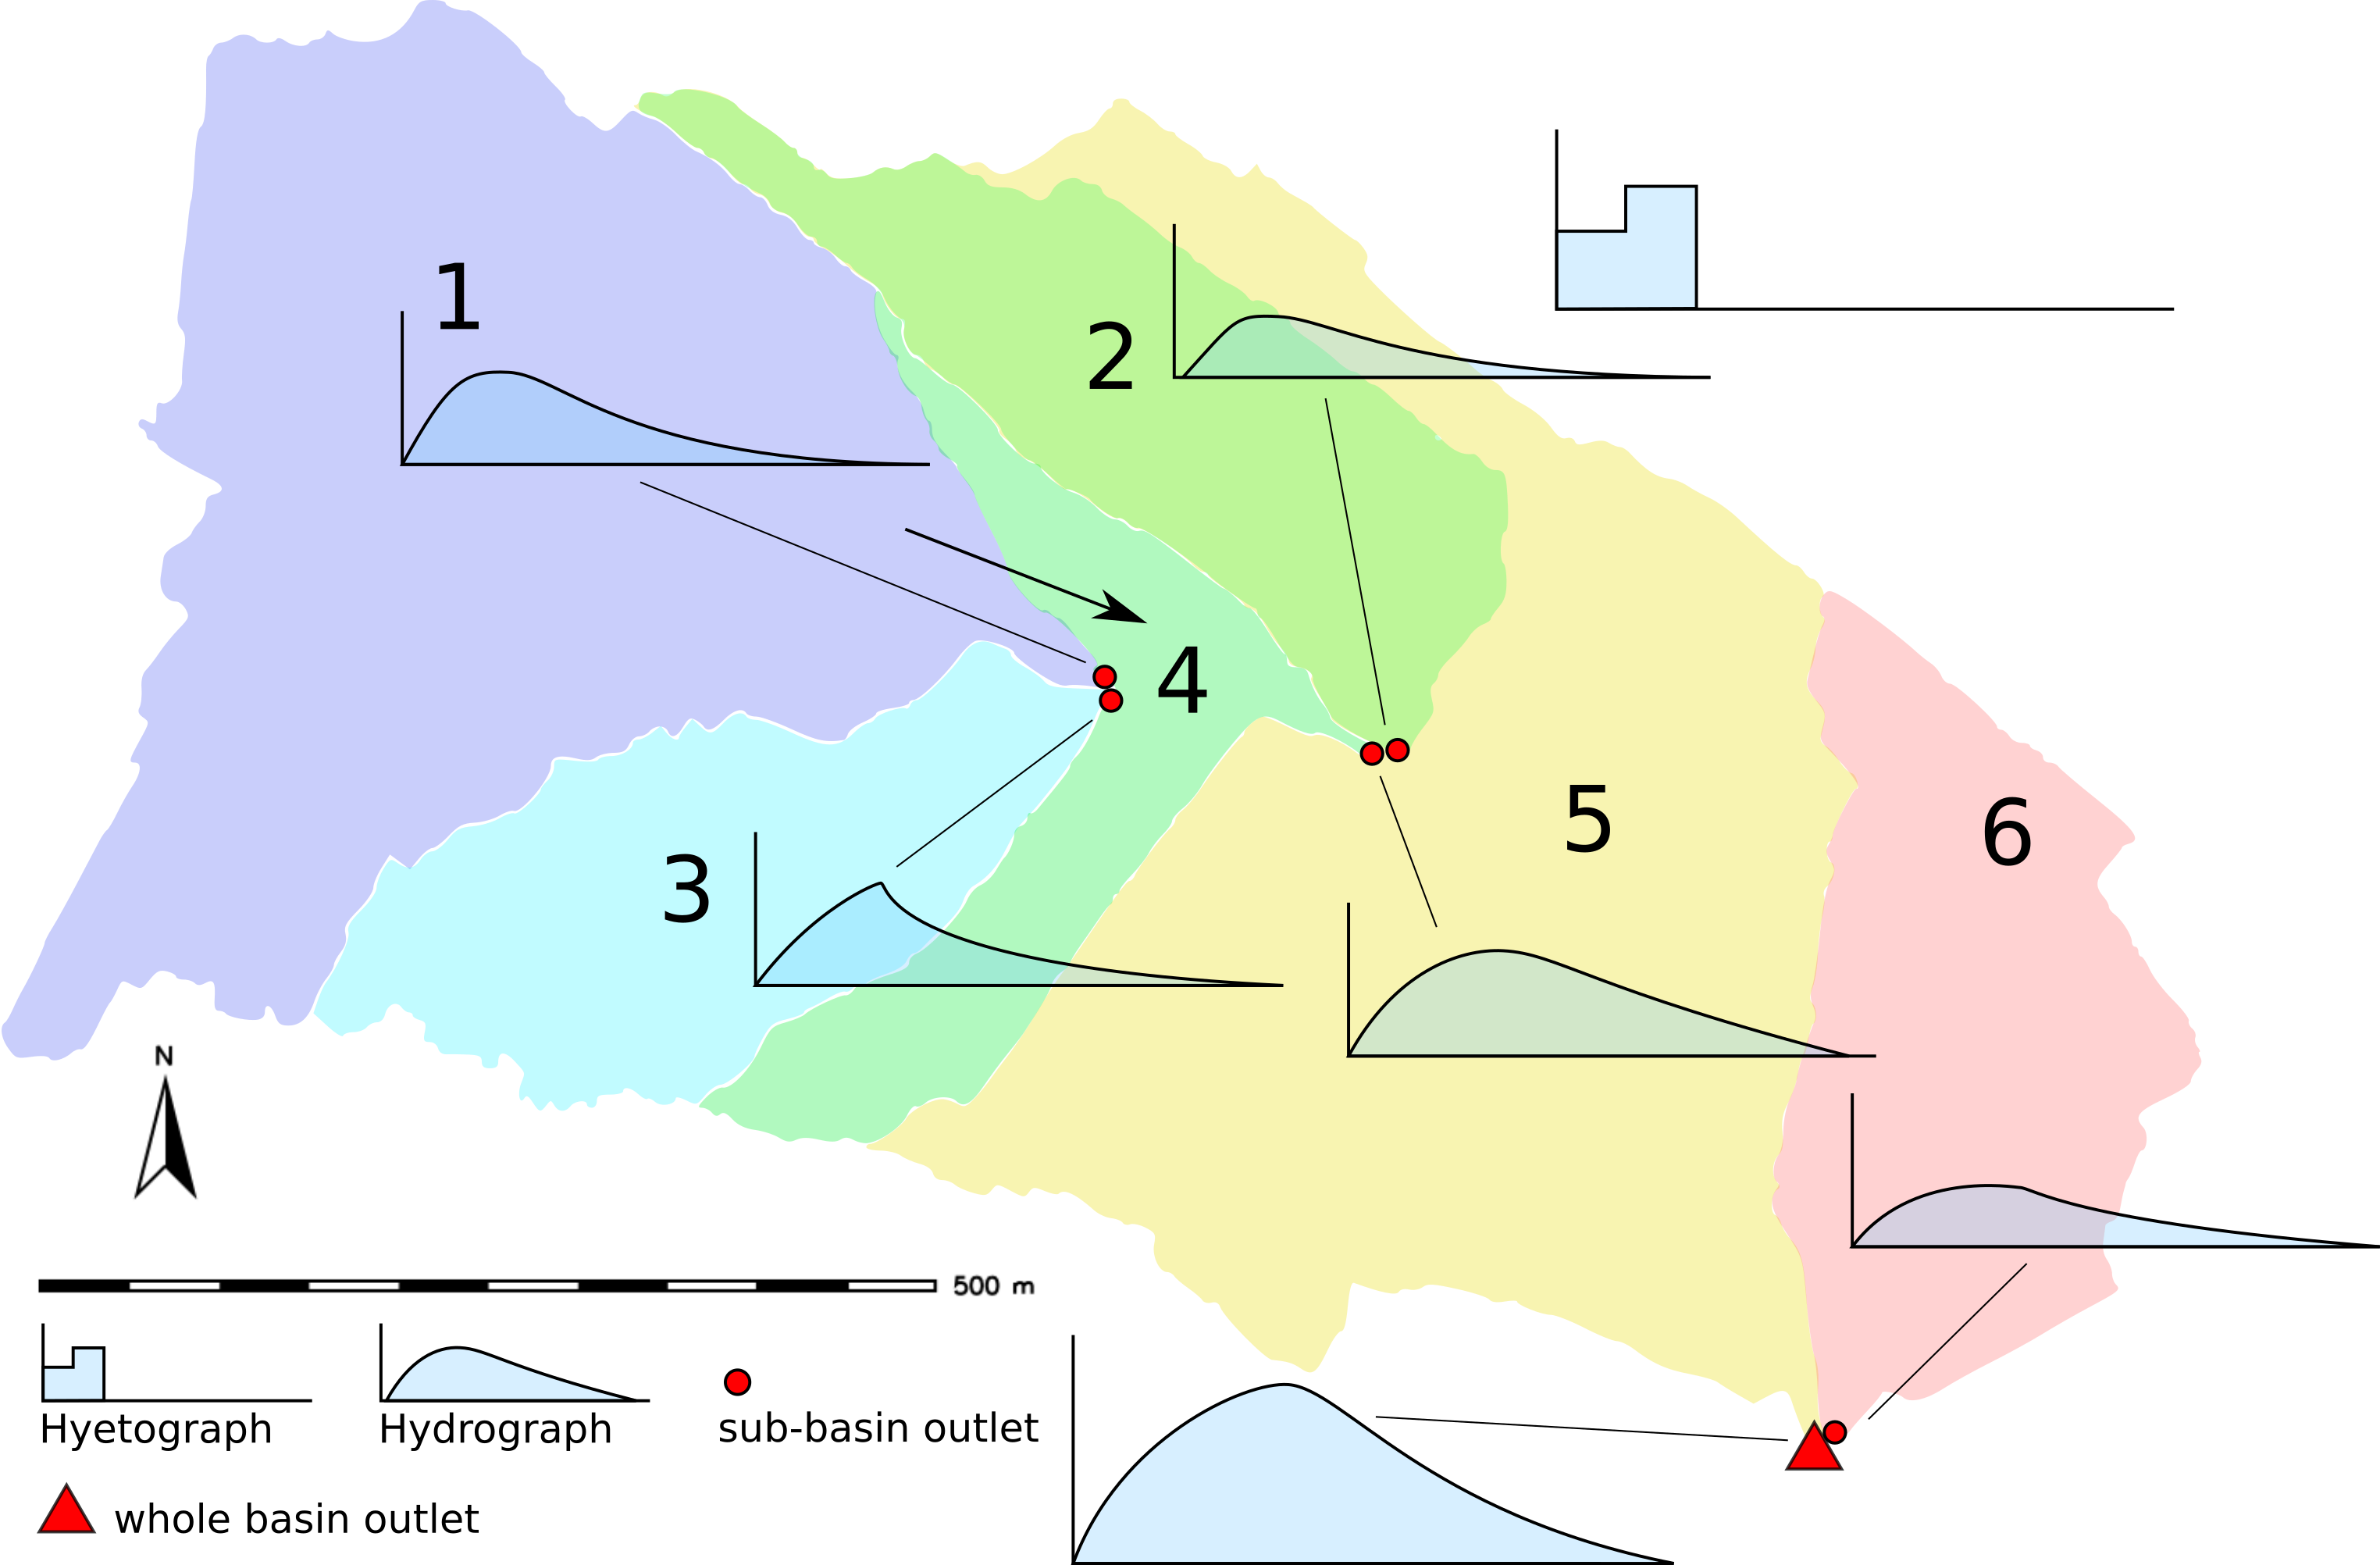
\includegraphics[width=1.0\columnwidth]{figures/smoderp-cpu-parallel.png}
    \caption{Strategy for CPU-parallelization}
    \label{fig:cpu-parallel}
  \end{center}
\end{figure}




